\tikzset{%
  % Specifications for style of nodes:
         base/.style = {rectangle, rounded corners, draw = black, minimum width=2.5cm, minimum height=1cm, fill=orange!15, font=\ttfamily},
}

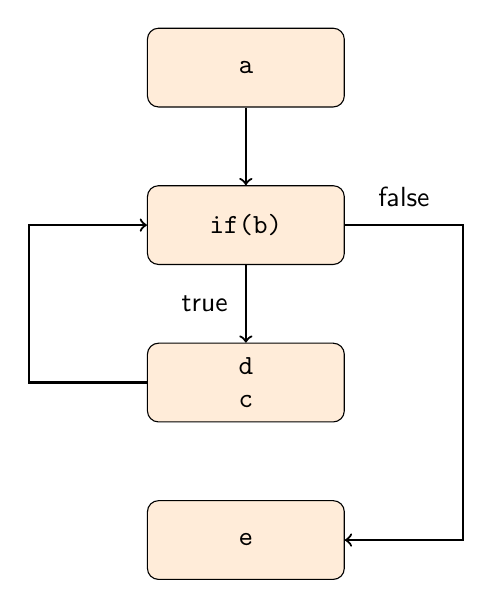
\begin{tikzpicture}[node distance=2cm, every node/.style={fill=white, font=\sffamily}, align=center]
    % Draw nodes
    \node (start)       [base]                        {a};
    \node (while)       [base, below of = start]      {if(b)};
    \node (code)        [base, below of = while]      {d\\c};
    \node (end)         [base, below of = code]       {e};

    % Draw arrows
    \draw[->,thick]           (start) -- (while);
    \draw[->,thick]           (while) -- node[left = 0.1cm, midway] {true} (code);

    \draw[->,thick]       (code.west) -- ++(-1.5,0) -- ++(0,2) -- ++(1.5,0)         (while);
    \draw[->,thick]       (while.east) -- node[above = 0.1cm, midway] {false} ++(1.5,0) -- ++(0,-4) -- ++(-1.5,0)     (end);


\end{tikzpicture}
